\documentclass{standalone}
\usepackage[utf8]{inputenc}
\usepackage[T1]{fontenc}
\usepackage{tikz}
\usepackage{pgfplots}
\pgfplotsset{compat=1.18}
\usetikzlibrary{positioning,fit,calc,intersections}

\makeatletter
\def\markxof#1{%
  \pgf@process{#1}%
  \pgfmathparse{%
    (\pgf@x/\pgfplotsunitxlength + \pgfplots@data@scale@trafo@SHIFT@x) / 10^\pgfplots@data@scale@trafo@EXPONENT@x%
  }%
}
\makeatother

\pgfplotsset{
  every axis/.append style={font=\small},
  customstyle/.style={%
    clip=true,
    axis x line=bottom,
    axis y line=left,
    xmin=0, xmax=40,
    samples=30,
    ymin=-1, ymax=5
  }
}

\begin{document}

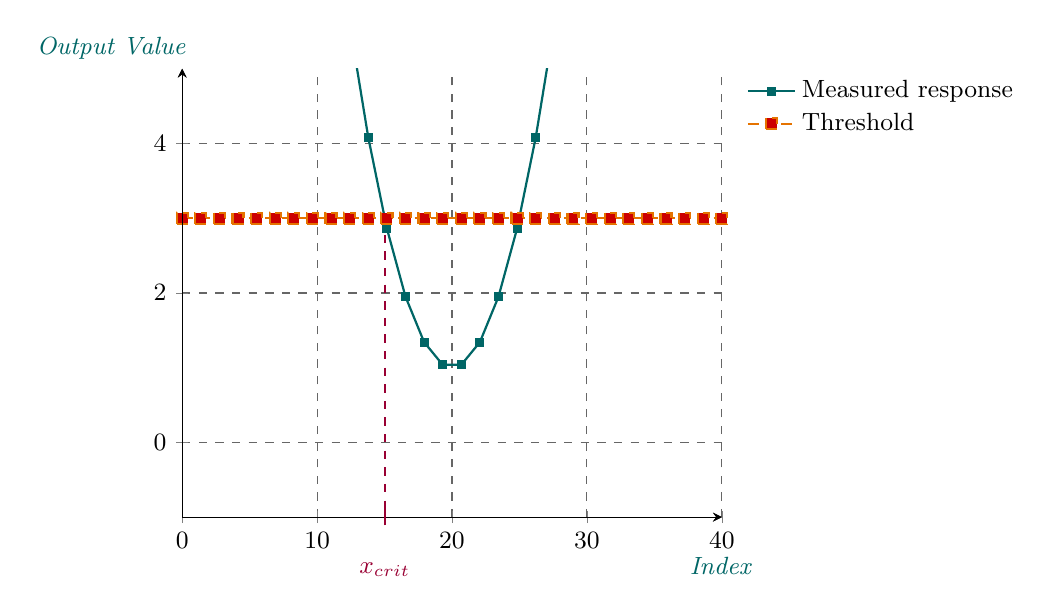
\begin{tikzpicture}
  \begin{axis}[
    customstyle,
    grid=major,
    grid style={dashed, line width=0.4pt, color=gray!80!black},
    xlabel={\emph{Index}},
    xlabel style={at={(1,-0.15)}, anchor=south, color=teal!80!black},
    ylabel={\emph{Output Value}},
    ylabel style={rotate=-90, at={(-0.13,1)}, anchor=south, color=teal!80!black},
    legend cell align=left,
    legend style={draw=none, font=\small, fill=none},
    legend pos=outer north east
  ]

    % Main plotted function: Parabola shifted and scaled
    \addplot+[name path global=main, teal!80!black, thick, mark=square*, mark options={fill=teal!80!black, scale=0.6}, domain=0:40, samples=30]
      {0.08*(\x-20)^2 + 1};

    % Reference line: horizontal
    \addplot+[name path global=ref, orange!90!black, thick, dash pattern=on 4pt off 2pt, domain=0:40]
      {3};

    % Find intersection
    \path [name intersections={of=main and ref, name=interx}];

    \pgfplotsextra{
      % Extract the first intersection's x-coordinate
      \path (interx-1) \pgfextra{\markxof{interx-1}\xdef\mytick{\pgfmathresult}};
    }

    % Dashed vertical from intersection
    \draw[thick, dashed, purple!80!black]
      (interx-1) -- ($(axis cs:0,-1)!(interx-1)!(axis cs:40,-1)$);

    \legend{Measured response, Threshold}
  \end{axis}

  % Overlay axis for extra tick
  \begin{axis}[
    customstyle,
    xtick=\empty, ytick=\empty,
    extra x ticks={\mytick},
    extra x tick labels={$x_{crit}$},
    extra x tick style={
      xticklabel style={yshift=-10, color=purple!80!black},
      major tick length=6pt,
      tick style={thick, color=purple!80!black}
    }
  ]
  \end{axis}
\end{tikzpicture}

\end{document}